\documentclass{standalone}
\usepackage{pgfplots}
\pgfplotsset{compat=1.18}
\usetikzlibrary{decorations.pathreplacing}

\begin{document}
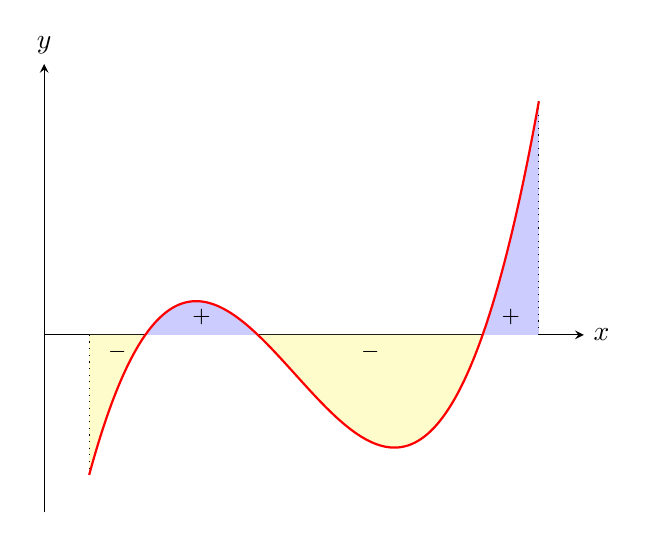
\begin{tikzpicture}
  \begin{axis}[
    axis lines=center,
    xlabel={\(x\)},
    ylabel={\(y\)},
    xlabel style={at={(ticklabel* cs:1)}, anchor=west},
    ylabel style={at={(ticklabel* cs:1)}, anchor=south},
    enlargelimits=true,
    axis line style={thin},
    xtick=\empty,
    ytick=\empty,
    black,
    ]

    \addplot[draw=none, fill=yellow!20, domain=0.5:1] {(x-1)*(x-2)*(x-4)} \closedcycle;
    \addplot[draw=none, fill=blue!20, domain=1:2] {(x-1)*(x-2)*(x-4)};
    \addplot[draw=none, fill=yellow!20, domain=2:4] {(x-1)*(x-2)*(x-4)};
    \addplot[draw=none, fill=blue!20, domain=4:4.5] {(x-1)*(x-2)*(x-4)} \closedcycle;
    \addplot[dotted, no markers] coordinates { (0.5,0) (0.5,-2.625) };
    \addplot[dotted, no markers] coordinates { (4.5,0) (4.5,4.375) };
    \addplot[thick, red, domain=0.5:4.5, smooth, samples=200] {(x-1)*(x-2)*(x-4)};

    \node[below] at (axis cs:0.75,0) {\footnotesize \(-\)};
    \node[above] at (axis cs:1.5,0) {\footnotesize \(+\)};
    \node[below] at (axis cs:3,0) {\footnotesize \(-\)};
    \node[above] at (axis cs:4.25,0) {\footnotesize \(+\)};

    \node[below,align=center] at (current axis.north) {\footnotesize };

  \end{axis}
\end{tikzpicture}
\end{document}
